\section{Distributed Architecture for Smart City}
\label{sec:Architecture}
%\vspace{0.10in}
Smart cities offer improved infrastructure for various public sector applications utilizing different technologies and devices. In a typical smart city environment, there are coherent data communications between heterogeneous entities and systems. To make better decisions, data integrity is vital along with security and confidentiality. To realize this scenario, in this section, we deploy Blockchain-based nodes in a smart city environment, Fig. \ref{fig:Main_Architecture} explains the architecture where different city departments (City HQ, Traffic and Police, Communications, Education and Healthcare) have several subsystems and IoTs that share data with their representative central servers. Each of these representative servers is a peer on the Blockchain network and responsible for sharing with other peers (Fig. \ref{fig:Sawtooth_Architecture}). To simplify the deployment process, we propose a methodology and simulate the smart city nodes and the network.

\begin{figure}[!ht] % H for place here
    \centering
    \setlength{\belowcaptionskip}{-10pt}
    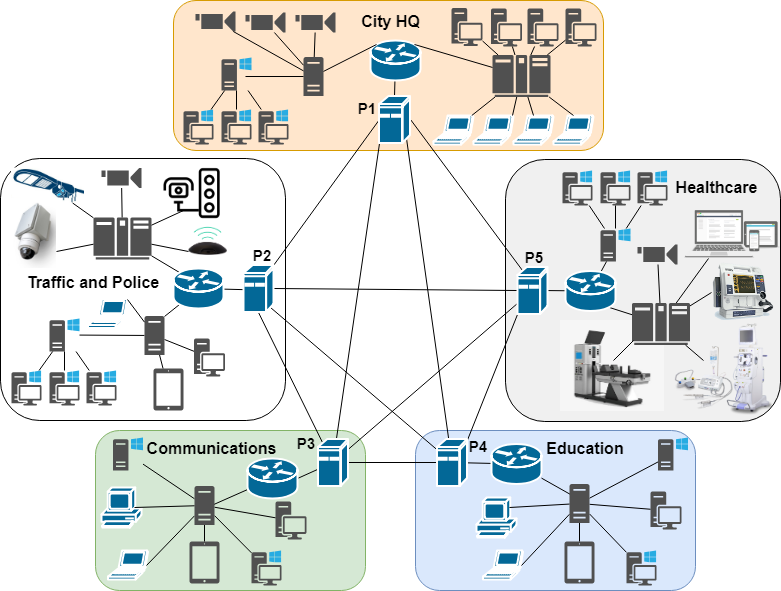
\includegraphics[scale=.30]{figs/main_arch.png}
    \caption{Smart City Environment Architecture}
    \label{fig:Main_Architecture} %refer the figure with this label
\end{figure}

\begin{figure*}[!ht] % ! force and t next page top
    \centering
    \setlength{\belowcaptionskip}{-10pt}
    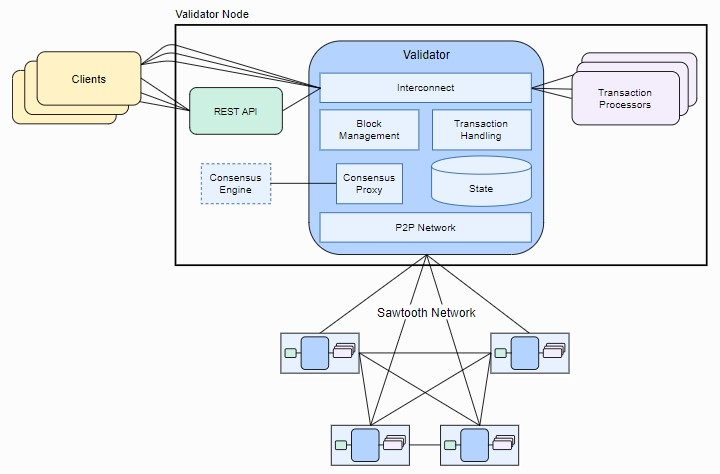
\includegraphics[width=5in]{figs/sawtooth_arch.png}
    \caption{Sawtooth Architecture \cite{sawtooth-architecture-guide}}
    \label{fig:Sawtooth_Architecture} %refer the figure with this label
\end{figure*}

\subsection{Methodology}
The nodes are deployed in the following fashion:

\textbf{(1) Genesis Node Deployment}: The first node on the Blockchain network contains the genesis block. Genesis block is the first block and the root of the Blockchain. This block does not contain any transactions. However, it contains the configuration settings which are used to bootstrap the very first validator node. The genesis block is then forwarded to the other peer nodes upon joining to the Blockchain network. Deployment and configuration of genesis node is a necessary prerequisite for allowing other validator nodes to join the Blockchain infrastructure.

\textbf{(2) Validator Nodes Deployment}: Any node joining the Blockchain network after the genesis node will initially connect to either the genesis node or any other fully functional peer in the Blockchain network to obtain the necessary information and settings about the genesis block. This deployment phase can run in parallel or sequentially. In each case, the genesis node has to be deployed first, and the rest of the validator nodes can be deployed sequentially or in parallel afterwards. Table I explains the total time taken by sequential and parallel deployments.

\begin{table}[H]
\centering
\label{tab:dep_times}
\begin{tabular}{|l|l|}
\hline
Deployment Type & Deployment Time   \\ \hline
Sequential      & 37min 53sec.      \\ \hline
Parallel        & 6min 42sec.       \\ \hline
\end{tabular}
\caption{Total deployment overheads.}
\vspace{-4mm}
\end{table}

To automate the deployment, we have created a deployment script\footnote{https://goo.gl/ic3Z1F} that allows a city IT administrator to deploy any number of validator nodes to establish the decentralized P2P network for running the ledger service easily. The script execution enables the user to select between deployment (Genesis/Validator node) and peering modes (Static/Dynamic). Fig. \ref{fig:script} explains the overall flow of the script functionality which is mainly divided into three main phases as highlighted in different colors. The phases are explained as below:

\begin{figure}[H] % H for place here
    \centering
    \setlength{\belowcaptionskip}{-10pt}
    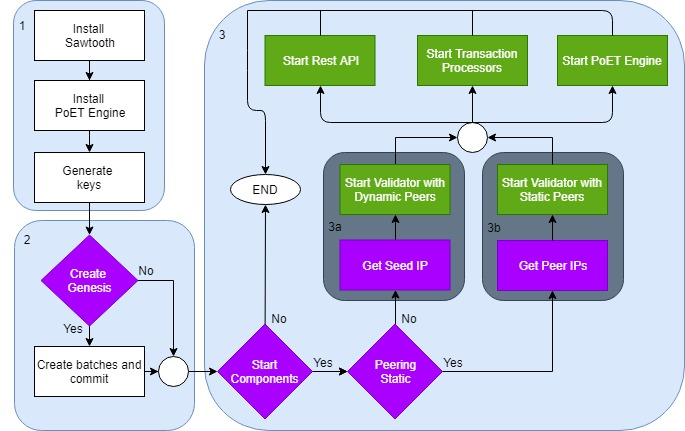
\includegraphics[scale=.60]{figs/block_diagram.png}
    \caption{Block diagram of the automation script}
    \label{fig:script} %refer the figure with this label
\end{figure}

\textbf{Phase 1: Sawtooth Deployment}: This phase runs on each node by default whenever the script is executed and deploys the required Sawtooth components.

\textbf{Phase 2: Genesis Block Creation}: This is an optional phase to deploy the genesis block with the chain configuration settings required for bootstraping validator nodes. In case of the first node, the user will pass ``Y'' as the first parameter to deploy the genesis block on the first node and ``N'' for the validator nodes to skip this phase.

\textbf{Phase 3: Starting Components}: This phase starts the Sawtooth components (Fig. \ref{fig:script} green boxes) that are required in order to bring the node up on the Sawtooth network. This phase is also optional, and the user can decide to run or skip this phase. In the case, if the user chooses to skip this phase, there is an additional script provided just for this phase to start the components. The additional script ``start\_components\_poet.sh'' instead of running the entire deployment process from the beginning, starts the components and takes peering options as parameters. The area highlighted grey (3a and 3b) in the Fig. \ref{fig:script} phase 3, is the peer/seed selection options (Dynamic or Static \cite{sawtooth-peering}) that allows the user to customize based on how the user wants the current node to peer up with the existing network. With dynamic peering, the new nodes can join without having to restart existing node's components or specifying IP addresses of existing nodes and in case of static peering, only pre-defined peers that can connect. For this phase, the user needs to pass three parameters (Param 2, 3 and 4 Table II).

\subsection{Deployment Categories}
This section discusses different deployment scenarios that we can have while simulating the Blockchain-based smart city infrastructure. Each scenario is explained further using a table containing user parameters that needs to be passed while initiating the deployment process. Fig. \ref{fig:peering} refers to the overall deployment of nodes.

\begin{figure}[H] % H for place here
    \centering
    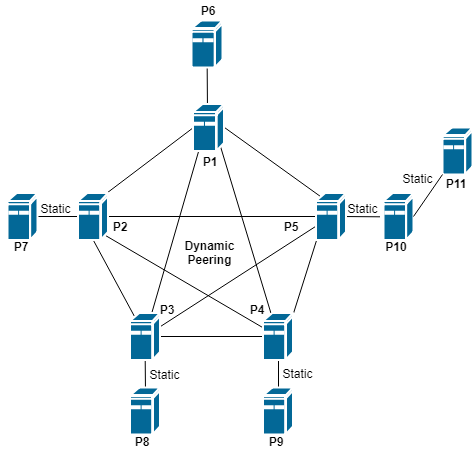
\includegraphics[scale=.5]{figs/peering.png}
    \setlength{\belowcaptionskip}{-5pt}
    \caption{Full network topology (Dynamic and Static peering)}
    \label{fig:peering} %refer the figure with this label
\end{figure}

\textbf{Scenario 1: First node (Genesis) deployment}: 
In this case, the user is trying to deploy the first node for the Blockchain network that will contain the genesis block. For this case, we assume that the user wants to start the components with the “Dynamic” peering mode. This scenario well suites for node ``P1'' (Fig. \ref{fig:peering}) under the City HQ department in the smart city simulation. 

For this scenario, the following parameters will be passed:
\begin{table}[H]
\centering
\label{tab:genesis_install}
\begin{tabular}{|l|l|}
\hline
Parameter 1: Create Genesis block? & Y         \\ \hline
Parameter 2: Start components      & Y         \\ \hline
Parameter 3: Peering static?       & N         \\ \hline
Parameter 4: Seed IP:              & tcp://current-machine-IP:port \\ \hline
\end{tabular}
\caption{Genesis node deployment.}
\vspace{-4mm}
\end{table}

Since this is the first node on the network, the seed IP will be the IP address of the current node. 

\textbf{Scenario 2: Validator node deployment (Known Genesis)}: 
In this case, the user is trying to deploy a peer node after the genesis node is up and running. The genesis node should be running with Dynamic peering mode actively looking for peers to connect. 
For this node, we are assuming that the user is aware of the IP address of the genesis node and wants to run the components under the ``Dynamic'' peering mode. This case can be applied to each departmental servers (Fig. \ref{fig:Main_Architecture} P2-P5).

For this scenario, the following parameters will be passed:
\begin{table}[H]
\centering
\label{tab:node_n_install}
\begin{tabular}{|l|l|}
\hline
Parameter 1: Create Genesis block? & N                          \\ \hline
Parameter 2: Start components      & Y                          \\ \hline
Parameter 3: Peering static?       & N                          \\ \hline
Parameter 4: Seed IP:              & tcp://genesis-node-ip:port \\ \hline
\end{tabular}
\caption{Validator node deployment - Known Genesis.}
\vspace{-4mm}
\end{table}
Since this is not the first node on the network, we will not create the genesis block on this node but provide the IP address of the seed, i.e. either the genesis node or any active peer that has already become a peer with the genesis node.

\textbf{Scenario 3 – Validator node deployment (Unknown Genesis)}: 
In this case, the user is trying to deploy a peer node after the genesis node is up and running and the user is not aware of the genesis node’s IP address. However, the IP address another active peer is known. As we see in Fig. \ref{fig:peering}, P10 is connected with P5 and similarly P11 with P10. For this case, we are assuming that these nodes are connecting with their neighbors under ``Dynamic'' peering mode. This scenario can apply to any node on the network which is not connected directly with the genesis node. 

For this scenario, the following parameters will be passed:
\begin{table}[H]
\centering
\label{tab:node_n_install2}
\begin{tabular}{|l|l|}
\hline
Parameter 1: Create Genesis block? & N                          \\ \hline
Parameter 2: Start components      & Y                          \\ \hline
Parameter 3: Peering static?       & N                          \\ \hline
Parameter 4: Provide seed(s) IP:   & tcp://seed-node-ip:port    \\ \hline
\end{tabular}
\caption{Validator node deployment - Unknown Genesis.}
\vspace{-4mm}
\end{table}

\textbf{Scenario 4 – Validator node deployment (Static peering)}: 
For this scenario, we are assuming the user wants to deploy a peer node with predefined fixed peers instead of dynamic. 

For this scenario, the following parameters will be passed:
\begin{table}[H]
\centering
\label{tab:node_n_install2}
\begin{tabular}{|l|l|}
\hline
Parameter 1: Create Genesis block? & N                          \\ \hline
Parameter 2: Start components      & Y                          \\ \hline
Parameter 3: Peering static?       & Y                          \\ \hline
Parameter 4: Provide peer(s) IP:   & tcp://peering-node-ip:port \\ \hline
\end{tabular}
\caption{Static node deployment.}
\vspace{-4mm}
\end{table}

For ``Static'' peering, port numbers are also required. If there are more than one static peers, they can be specified with a comma, e.g.: ``tcp://peering-node1-IP:port\#,tcp://peering-node2-IP:port\#,...''

\textbf{Test Scenario 5 – Churning validator node deployment}: 
Any node on the network can go down at any point. In this case, an existing peer, e.g. P3 (Fig. \ref{fig:peering}) from the Blockchain network goes offline for some period and comes back online. We are assuming that the user will start the components under dynamic peering mode in this case.

For this scenario, the following parameters will be passed:
\begin{table}[H]
\centering
\label{tab:node_n_install2}
\begin{tabular}{|l|l|}
\hline
Parameter 1: Create Genesis block? & N                          \\ \hline
Parameter 2: Start components      & Y                          \\ \hline
Parameter 3: Peering static?       & N                          \\ \hline
Parameter 4: Provide peer(s) IP:   & tcp://active-peer-ip:port  \\ \hline
\end{tabular}
\caption{Churning node deployment.}
\vspace{-4mm}
\end{table}

In Fig. \ref{fig:peering}, it is seen that node P3 is acting as a peer node for P8 as well, and the downtime for P3 isolates the P8 node from the Blockchain network. Similarly downtime for P5 isolates P10 and P11 from the entire network. In the next section, we will discuss and evaluate all of the above scenarios to find out the outcome. 
